% ============================================================
%  Поглавље 2: Квантно рачунарство и две главне парадигме
% ============================================================
\section{Квантно рачунарство и различите парадигме}
\label{sec:np}

Квантно рачунарство данас није јединствена архитектура него породица
различитих рачунских парадигми, свака са сопственим физичким темељима,
математичким формализмом и класом проблема за коју је најподесније.
У овом поглављу представљамо две доминантне парадигме које су релевантне
за решавање оптимизационих проблема: \textbf{квантно рачунарство засновано
на колима} и \textbf{квантно жарење}.

% ============================================================
\subsection{Заједничке основе: кубити и суперпозиција}
% ============================================================



Обе парадигме заснивају се на кубиту, квантном аналогу класичног бита.
Стање $n$ кубита описује се вектором у Хилбертовом простору
$\mathcal{H} = (\mathbb{C}^2)^{\otimes n}$ димензије $2^n$:
\[
  |\psi\rangle = \sum_{x \in \{0,1\}^n} \alpha_x |x\rangle, \qquad
  \sum_{x} |\alpha_x|^2 = 1.
\]
Кубит када му се измери вредност може бити само $|0\rangle$ или $|1\rangle$, али пре мерења може бити у суперпозицији свих могућих конфигурација.
На пример кубит у стању $|\psi\rangle = \frac{|0\rangle + |1\rangle}{\sqrt{2}}$ има једнаку вероватноћу да се измери као $|0\rangle$ или $|1\rangle$.
Двокубитни систем у стању $|\psi\rangle = \frac{|00\rangle + |11\rangle}{\sqrt{2}}$ је у суперпозицији стања $|00\rangle$ и $|11\rangle$, али никада неће бити измерен као $|01\rangle$ или $|10\rangle$.
Ова стања одговарају појединачним битовима у класичном рачунарству, али једина разлика је што ми не знамо унапред колика
је вредност сваког бита у стварности све док не измеримо систем.

Суперпозиција омогућује да систем истовремено ``буде'' у свим $2^n$
конфигурацијама пре мерења, управо то чини квантно рачунарство
концептуално различитим од класичног.

% ============================================================
\subsection{Парадигма I: Квантна кола (Gate-Based QC)}
% ============================================================


\subsubsection{Принцип рада}

У моделу квантних кола, рачунање се изводи применом секвенце
\emph{квантних капија},  унитарних трансформација $U$, на почетно
стање $|0\rangle^{\otimes n}$:
\[
  |\psi_{\text{out}}\rangle = U_L \cdots U_2 U_1 \,|0\rangle^{\otimes n}.
\]
Овај израз представља квантно коло са $L$ капија. Које делује на регистар са  $n$ кубита, и примењеује различите трансформације на њега.
Коначни одговор добија се мерењем, које стање пројектује на неки
базни вектор са одређеном вероватноћом.

\subsubsection{Базичне квантне капије}

Свака квантна капија је \emph{унитарна} трансформација ($U U^\dagger = I$),
чиме је рачунање реверзибилно. Матричне репрезентације основних капија:
\[
  H = \frac{1}{\sqrt{2}}\begin{pmatrix}1 & 1\\ 1 & -1\end{pmatrix}, \qquad
  X = \begin{pmatrix}0 & 1\\ 1 & 0\end{pmatrix}, \qquad
  R_Z(\theta) = \begin{pmatrix}e^{-i\theta/2} & 0\\ 0 & e^{i\theta/2}\end{pmatrix}, 
\]

\paragraph{Просте капије (један кубит).}
На слици~\ref{fig:simple-gates} приказано је шест основних
једнокубитних капија. Поред матрица $H$, $X$ и $R_Z$ из горњег
израза, додајемо:
\[
  Y = \begin{pmatrix}0&-i\\i&0\end{pmatrix}, \qquad
  S = \begin{pmatrix}1&0\\0&i\end{pmatrix}, \qquad
  T = \begin{pmatrix}1&0\\0&e^{i\pi/4}\end{pmatrix}, \qquad
  R_Y(\theta) = \begin{pmatrix}\cos\frac{\theta}{2}&-\sin\frac{\theta}{2}\\\sin\frac{\theta}{2}&\cos\frac{\theta}{2}\end{pmatrix}.
\]

\begin{figure}[h]
\centering
\begin{quantikz}
  \lstick{$|q\rangle$} & \gate{H} & \qw & \rstick{\small $\tfrac{|0\rangle\pm|1\rangle}{\sqrt{2}}$}
\end{quantikz}
\quad
\begin{quantikz}
  \lstick{$|q\rangle$} & \gate{X} & \qw & \rstick{\small $|1{\oplus}q\rangle$}
\end{quantikz}
\quad
\begin{quantikz}
  \lstick{$|q\rangle$} & \gate{Y} & \qw & \rstick{\small $iY|q\rangle$}
\end{quantikz}

\vspace{0.6em}

\begin{quantikz}
  \lstick{$|q\rangle$} & \gate{S} & \qw & \rstick{\small $e^{i\pi/2}$ на $|1\rangle$}
\end{quantikz}
\quad
\begin{quantikz}
  \lstick{$|q\rangle$} & \gate{T} & \qw & \rstick{\small $e^{i\pi/4}$ на $|1\rangle$}
\end{quantikz}
\quad
\begin{quantikz}
  \lstick{$|q\rangle$} & \gate{R_Y(\theta)} & \qw & \rstick{\small реална ротација}
\end{quantikz}

\caption{Једнокубитне капије: Хадамар ($H$), Паули-$X$, Паули-$Y$,
         фазна ($S$), $\pi/8$ капија ($T$) и ротација $R_Y(\theta)$.}
\label{fig:simple-gates}
\end{figure}

\paragraph{Двокубитне капије.}
Двокубитне капије делују на пар кубита и могу генерисати заплетеност.
Три кључне:

\begin{figure}[h]
\centering
\begin{quantikz}
  \lstick{$|c\rangle$} & \ctrl{1} & \qw & \rstick{$|c\rangle$} \\
  \lstick{$|t\rangle$} & \targ{}  & \qw & \rstick{$|t\oplus c\rangle$}
\end{quantikz}
\qquad
\begin{quantikz}
  \lstick{$|c\rangle$} & \ctrl{1}   & \qw & \rstick{$(-1)^{ct}|c\rangle$} \\
  \lstick{$|t\rangle$} & \control{} & \qw & \rstick{$(-1)^{ct}|t\rangle$}
\end{quantikz}
\qquad
\begin{quantikz}
  \lstick{$|a\rangle$} & \swap{1} & \qw & \rstick{$|b\rangle$} \\
  \lstick{$|b\rangle$} & \targX{} & \qw & \rstick{$|a\rangle$}
\end{quantikz}
\caption{Двокубитне капије: CNOT (controlled-NOT), CZ (controlled-$Z$)
         и SWAP (размена стања кубита).}
\label{fig:two-qubit-gates}
\end{figure}

\paragraph{Трокубитна Тофолијева капија (CCNOT).}
Тофолијева капија примењује $X$ на циљни кубит само ако су
\emph{оба} управљачка у стању $|1\rangle$.
Будући да реализује NAND операцију, она је функционално потпуна
и доказује да квантна кола могу симулирати произвољно класично рачунање.

\begin{figure}[h]
\centering
\begin{quantikz}
  \lstick{$|a\rangle$} & \ctrl{1} & \qw & \rstick{$|a\rangle$} \\
  \lstick{$|b\rangle$} & \ctrl{1} & \qw & \rstick{$|b\rangle$} \\
  \lstick{$|t\rangle$} & \targ{}  & \qw & \rstick{$|t \oplus (a \wedge b)\rangle$}
\end{quantikz}
\caption{Тофолијева (CCNOT) капија: $X$ се примењује на $|t\rangle$
         само када су $|a\rangle = |b\rangle = |1\rangle$.}
\label{fig:toffoli}
\end{figure}

Оно што можемо да приметимо да нема неке велике разлике између ових капија и класичних логичких капија
на дијаграмима, али је битно да су ове капије реверзибилне, што значи да не губе информацију и да се могу изводити уназад.
Ово је кључна разлика у односу на класичне логичке капије које нису реверзибилне (нпр. AND, OR, NAND). У квантном рачунарству,
реверзибилност је неопходна јер унитарне трансформације морају имати инверз.

Класична AND капија је типичан пример \emph{иреверзибилне} операције.
Она пресликава два улазна бита у један излазни, чиме неповратно губи
информацију. Из излазне вредности $0$ не може се одредити да ли је улаз
био $(0,0)$, $(0,1)$ или $(1,0)$ --- три различите улазне комбинације
дају исти излаз. Таква функција није инјекција и не поседује инверз,
па се не може реализовати унитарном матрицом.

\begin{figure}[h]
\centering
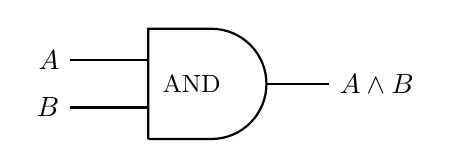
\begin{tikzpicture}[scale=1.0]
  % AND gate body: flat left side, semicircular right side
  \draw[thick] (0,0) -- (0,1.4) -- (0.8,1.4)
        arc[start angle=90, end angle=-90, radius=0.7]
        -- (0,0);
  % Input wires
  \draw[thick] (-1.0,1.0) -- (0,1.0) node[left, at start] {$A$};
  \draw[thick] (-1.0,0.4) -- (0,0.4) node[left, at start] {$B$};
  % Output wire
  \draw[thick] (1.5,0.7) -- (2.3,0.7) node[right] {$A \wedge B$};
  % Gate label
  \node at (0.55,0.7) {\small AND};
\end{tikzpicture}
\qquad\qquad
% Truth table
\begin{tabular}[b]{cc|c}
  \toprule
  $A$ & $B$ & $A \wedge B$ \\
  \midrule
  0 & 0 & 0 \\
  0 & 1 & 0 \\
  1 & 0 & 0 \\
  1 & 1 & 1 \\
  \bottomrule
\end{tabular}
\caption{AND капија и њена таблица истинитости. Три улазне комбинације
  $(0,0)$, $(0,1)$ и $(1,0)$ дају исти излаз $0$, па функција
  није инјекција, информација о улазу се губи и операција
  није реверзибилна.}
\label{fig:and-gate}
\end{figure}

\subsubsection{Хардверске платформе}

Неколико компанија данас нуди комерцијално доступне квантне рачунаре
засноване на колима:

\textbf{IBM Quantum} користи суперпроводљиве кубите охлађене близу
апсолутне нуле (${\sim}15\,\mathrm{mK}$). Кроз платформу IBM Quantum
Experience корисници могу покретати програме написане у Qiskit-у
директно на стварном хардверу. Серија Eagle/Heron процесора достигла
је преко 1000 физичких кубита (Condor, 2023), мада је број грешака
и даље ограничавајући фактор.

\textbf{Google Quantum AI} такође гради суперпроводљиве процесоре.
Чип Sycamore (54 кубита, 2019) коришћен је у демонстрацији
,,квантне надмоћи'', задатку за који је тврђено да класичном
рачунару треба 10.000 година, а процесор га је решио за 200 секунди
(тврдња је касније оспорена у литератури).
Новији чип Willow (2024) показује напредак у корекцији грешака.

\textbf{IonQ} ради на бази заробљених јона (trapped-ion технологија):
атоми итербијума одржавају се у вакуумској замци електромагнетним
пољем, а капије се примењују ласерским пулсовима. Иако су тренутно
спорији од суперпроводљивих система, кохеренције јони имају знатно
нижу стопу грешака и дуже вријеме кохеренце.

\textbf{Quantinuum} (спој Honeywell Quantum Solutions и Cambridge
Quantum) такође примењује приступ заробљених јона и истиче се међу
највишим вредностима квантног волумена --- мере која узима у обзир
број кубита, повезаност и стопу грешака истовремено.

\textbf{Остали актери.} Компаније попут Rigetti (суперпроводљивост),
PsiQuantum (фотонски кубити) и Intel (silicon spin qubits) истражују
алтернативне физичке имплементације у потрази за скалабилнијим решењем.

\subsubsection{Ограничења у NISQ ери}


Тренутни квантни рачунари са колима налазе се у такозваној
\textit{NISQ ери}~\cite{preskill2018} (Noisy Intermediate-Scale Quantum):
имају 50--1000 кубита, али су подложни грешкама и немају потпуну
корекцију грешака. Дубина кола ограничена је временом декохеренције.

% ============================================================
\subsection{Парадигма II: Квантно жарење (Quantum Annealing)}
% ============================================================

% --- Опис ---
% Квантно жарење је специјализована парадигма за оптимизационе
% проблеме. Инспирисана је класичним симулираним жарењем, али
% користи квантно тунелирање уместо термалних флуктуација.

\subsubsection{Класично симулирано жарење}

Симулирано жарење (Kirkpatrick et al., 1983) је метахеуристички
алгоритам инспирисан процесом физичког жарења метала: загревање
уклања дефекте у кристалној решетки, а споро хлађење омогућује
систему да нађе нискоенергетско стање.

\textbf{Идеја алгоритма.} Циљ је минимизовати функцију цене $E(s)$
над дискретним простором стања $s$. У свакој итерацији алгоритам:
\begin{enumerate}[leftmargin=*, label=\arabic*.]
  \item предложи мали случајни помак у суседно стање $s'$;
  \item ако је $E(s') < E(s)$, прихвати помак безусловно;
  \item ако је $E(s') \geq E(s)$, прихвати помак са вероватноћом
        $P = e^{-\Delta E / T}$, где је $\Delta E = E(s') - E(s)$
        и $T$ тренутна ``температура''.
\end{enumerate}
Температура се постепено смањује по \emph{распореду хлађења}
(нпр. $T_k = T_0 / \log(1+k)$). Висока температура на почетку
омогућује велике скокове преко лоших локалних решења; ниска
температура на крају усмерава претрагу ка финалном минимуму.

\textbf{Ограничење.} Класично жарење прескаче баријере искључиво
захваљујући температурним флуктуацијама. Уска, висока баријера
захтева велику температуру --- а висока температура истовремено
деградира прецизност финалног решења. Овај компромис отежава
проналажење глобалног минимума у пејзажима са бројним уским
локалним минимумима.

\subsubsection{Принцип рада}

Идеја квантног жарења потиче из аналогије са класичним
\emph{симулираним жарењем} (Kirkpatrick et al., 1983), али уместо
термалних флуктуација користи \emph{квантно тунеловање} — способност
квантног система да пролази кроз енергетске баријере уместо да их
прескаче. Ово је кључна предност над класичним жарењем када
енергетски пејзаж има бројне уске, дубоке локалне минимуме.

\textbf{Почетни Хамилтонијан} $\hat{H}_0$ бира се тако да му је
основно стање лако за припремити. Стандардан избор је попречно
магнетно поље:
\[
  \hat{H}_0 = -\sum_{i=1}^n \hat{X}_i,
\]
чије је основно стање равномерна суперпозиција свих $2^n$ стања,
$|+\rangle^{\otimes n}$.

\textbf{Проблемски Хамилтонијан} $\hat{H}_P$ кодира функцију коју
оптимизујемо: његово основно стање одговара оптималном решењу.
За QUBO/Изинг проблеме:
\[
  \hat{H}_P = \sum_{i} h_i \hat{Z}_i + \sum_{i < j} J_{ij} \hat{Z}_i \hat{Z}_j.
\]

\textbf{Адијабатска еволуција.} Систем се спором линеарном
интерполацијом води из $\hat{H}_0$ у $\hat{H}_P$:
\[
  \hat{H}(t) = \left(1 - \frac{t}{T}\right)\hat{H}_0
             + \frac{t}{T}\,\hat{H}_P, \qquad t \in [0, T].
\]
У тренутку $t = 0$ систем је у основном стању $\hat{H}_0$.
На крају ($t = T$) мерење даје стање блиско основном стању $\hat{H}_P$,
тј.\ (приближно) оптималном решењу.

\begin{theorem}[Адијабатска теорема]
Нека је $\Delta(t) = E_1(t) - E_0(t) > 0$ спектрални јаз
(разлика енергија основног и првог побуђеног стања у тренутку $t$).
Ако је укупно време жарења $T$ довољно велико у односу на
\[
  T \;\gg\; \frac{\max_t \|\partial_t \hat{H}(t)\|}{\min_t \Delta(t)^2},
\]
систем иницијализован у основном стању $\hat{H}_0$ остаје у
тренутном основном стању током целог процеса жарења.
\end{theorem}

\begin{remark}
Кључни изазов адијабатског рачунарства јесте \emph{спектрални јаз}:
ако $\Delta(t)$ постане веома мали током еволуције, потребно је
експоненцијално велико $T$, чиме се предност губи.
За НП-тешке проблеме очекује се да минимални јаз опада
полиномски или чак експоненцијално са величином инстанце.
\end{remark}

\textbf{Квантно тунелирање.} За разлику од класичног жарења које
„прескаче" преко баријере захваљујући температури, квантни систем
тунелира \emph{кроз} баријеру захваљујући суперпозицији.
Уска, висока баријера коју класично жарење тешко прелази може
бити прозирна за квантно тунелирање, па квантно жарење може
ефикасније наћи глобални минимум у одређеним пејзажима.

На слици~\ref{fig:annealing-schedule} приказан је типичан
распоред жарења: попречно поље $\Gamma(t)$ постепено слаби,
а проблемски члан $\lambda(t)$ јача.

\begin{figure}[h]
\centering
\begin{tikzpicture}[scale=1.1]
  \draw[->] (0,0) -- (5.2,0) node[right] {$t/T$};
  \draw[->] (0,0) -- (0,2.4) node[above] {амплитуда};
  % Gamma(t) = 1 - t/T (poprecno polje opada)
  \draw[blue!70!black, thick] (0,2) -- (5,0)
        node[right, blue!70!black] {$\Gamma(t) = 1 - t/T$};
  % lambda(t) = t/T (problemski clan raste)
  \draw[red!70!black, thick, dashed] (0,0) -- (5,2)
        node[right, red!70!black] {$\lambda(t) = t/T$};
  % ose
  \foreach \x/\l in {0/{$0$}, 2.5/{$T/2$}, 5/{$T$}}
    \draw (\x,0.05) -- (\x,-0.05) node[below] {\l};
  \foreach \y in {1,2}
    \draw (0.05,\y) -- (-0.05,\y) node[left] {$\y$};
\end{tikzpicture}
\caption{Распоред жарења: попречно поље $\Gamma(t)$ (квантне флуктуације)
         постепено слаби, а проблемски члан $\lambda(t)$ јача.
         На крају ($t = T$) доминира $\hat{H}_P$.}
\label{fig:annealing-schedule}
\end{figure}

\subsubsection{QUBO формулација}

% --- QUBO ---
% Квантно жарење природно решава QUBO проблеме.
% QUBO: minimize x^T Q x, x ∈ {0,1}^n.
% Исинговом трансформацијом (z = 2x-1) добија се Изингов модел
% директно реализован у хардверу.

Природни улазни формат за квантне жараче је
\textbf{QUBO} (Quadratic Unconstrained Binary Optimization):
\[
  \min_{\mathbf{x} \in \{0,1\}^n} \;\mathbf{x}^\top Q\, \mathbf{x},
  \qquad Q \in \mathbb{R}^{n \times n}.
\]

Супституцијом $z_i = 2x_i - 1 \in \{-1,+1\}$ добија се еквивалентни
\emph{Изингов модел}, директно реализован у хардверу квантног жарача:
\[
  \hat{H}_P = \sum_{i} h_i \hat{Z}_i + \sum_{i < j} J_{ij} \hat{Z}_i \hat{Z}_j.
\]


\subsubsection{Хардвер: D-Wave}

D-Wave Systems је тренутно једини комерцијални произвођач квантних
жарача. Њихов процесор \textbf{Advantage} (2020) садржи преко 5000
суперпроводљивих кубита охлађених на ${\sim}15\,\mathrm{mK}$, а
генерација \textbf{Advantage2} (у развоју) циља преко 7000 кубита са
побољшаним графом повезаности.

\textbf{Архитектура повезаности.}
Кубити нису потпуно повезани --- хардверски граф је реалан и редак
(sparse). Процесор Advantage користи \emph{Pegasus} граф у коме је
сваки кубит директно повезан са највише 15 суседа, за разлику од
старије \emph{Chimera} архитектуре (максимум 6 веза по кубиту).

\textbf{Уграђивање (Embedding).}
Пошто произвољан проблемски граф обично није подграф Pegasus-а,
неопходно је \emph{уграђивање}: логички кубит проблема представља
се ланцем физичких кубита везаних јаком феромагнетном везом.
Уграђивање може значајно повећати стварни број потребних физичких
кубита и представља практично ограничење за велике инстанце.

\textbf{Облачни приступ и примене.}
D-Wave нуди приступ преко \emph{Leap} облачне платформе са Python
библиотеком \texttt{dwave-ocean-sdk}. Међу познатим применама истичу
се: оптимизација рутирања возила (Volkswagen), финансијско
портфолио управљање и проблеми распоређивања у логистици.

% ============================================================
\subsection{Поређење парадигми}
% ============================================================

% TODO: Табела поређења:
% | Особина          | Кола (Gate-Based) | Жарење (Annealing) |
% |------------------|-------------------|--------------------|
% | Модел            | Унитарна кола     | Адијабатска еволуција|
% | Улаз             | Квантни програм   | QUBO/Изинг матрица |
% | Излаз            | Мерење на крају   | Основно стање      |
% | Платформе        | IBM, Google, IonQ | D-Wave             |
% | Намена           | Универзалан       | Оптимизација       |
% | Кубити (2024)    | ~1000 (физички)   | >5000              |
% | Корекција грешака| У развоју         | Не постоји         |

\begin{table}[ht]
  \centering
  \caption{Поређење две главне квантне парадигме.}
  \label{tab:paradigme}
  \renewcommand{\arraystretch}{1.3}
  \begin{tabular}{lll}
    \toprule
    \textbf{Особина}         & \textbf{Кола (Gate-Based)} & \textbf{Жарење (Annealing)} \\
    \midrule
    Рачунски модел           & Унитарна кола              & Адијабатска еволуција \\
    Улазни формат            & Квантни програм            & QUBO / Изингов модел \\
    Платформе                & IBM, Google, IonQ          & D-Wave \\
    Примарна намена          & Универзалан                & Комбинаторна оптимизација \\
    Број кубита (2024)       & ${\sim}1000$ физичких      & ${>}5000$ \\
    Корекција грешака        & У развоју                  & Не постоји \\
    \bottomrule
  \end{tabular}
\end{table}

Иако се парадигме разликују у механизму, оне нису потпуно раздвојене:
QAOA алгоритам са колима, инспирисан је
управо адијабатским жарењем и решава исте QUBO проблеме.
